%!TEX root = Main.tex
% Project analysis: words
\chapter{Project Evaluation and Reflection} % (fold)
\label{cha:project_analysis}

This chapter presents an analysis of the final solution, evaluating its primary strengths and weaknesses, and the progress as a whole.

\section{Analysis of Solution} % (fold)
\label{sec:analysis_of_solution}

	\subsection{The FPGA} % (fold)
	\label{sub:analysis_the_fpga}
		The FPGA used was very small, and the full required design could not fit on it.  In particular, the size of the model had to be reduced, so that each Gaussian mean and variance had fewer than 25 components, and not all 7000 senones were processed.  However, what has been implemented is adequate to prove the concept, and demonstrate the advantages gained from using an FPGA.  In addition, it was known from the start that the full model would never fit, and so although this is a practical limitation, it does not make the project less worthwhile.

		Various benchmarks have been presented in the form of timing data.  It was shown that the FPGA was capable of calculating senone scores far faster than the traditional processor, albeit with an acceptable loss of accuracy.  This is similar to results achieved by Melnikoff \cite{melnikoff2003speech} and Speech Silicon \cite{schuster2006speech}, and supports the principle that custom-made hardware is faster than general purpose processors.  For real-time speech recognition, getting the senone scores as fast as possible is very important, as it allows more time for decoding tasks.  Thus, using an FPGA may be beneficial, especially in embedded systems.  It is possible to extrapolate, from the data gathered, the system speed when a larger model is implemented.  If the full model (7000 senones, 25 components) was used, the scores would be computed in about 3.5ms, leaving 6.5ms (of a 10ms window) for pre-processing and decoding (this excludes communications time).  If the embedded process was used to calculate the scores, it would take % TODO!!!! Recompile GDP-in-C with N_COMPS=25

		A big disadvantage of using an FPGA, in such a system, is the need to communicate to it.  The communication is an added step that adds time to the senone scoring process, and, if it is not fast enough, may render the use of an FPGA not worthwhile.  The implemented communication method (UART) is extremely slow and is the weakest point of the system, as is obvious in Figure~\ref{fig:full_cycle} which shows a complete cycle of the top level state machine.  Although it is not visible, the state machine goes through PROC and GDP, but these stages are far faster than the UART communication.  UART was used primarily for the ease of implementation, and because at this stage real-time operations are not required.  However, for this system to be realistically useful, a better communication method needs to be developed -- either a far faster serial bus or some form of hybrid serial-parallel connection.

		\begin{figure}[tb]
			\begin{center}
				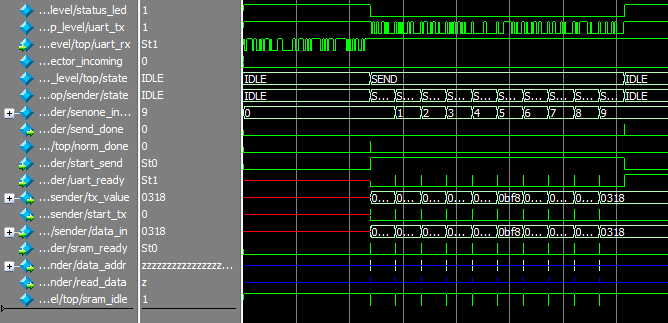
\includegraphics[width=\textwidth]{testbenches/full_cycle}
			\end{center}
			\caption{Simulation waveforms showing a full cycle of the top level state machine}
			\label{fig:full_cycle}
		\end{figure}

		% Additionally, the number format used caused the calculation accuracy to be reduced
	% subsection the_fpga (end)

	% Evaluate the speed - how long did each cycle take.  How much time was added by adding another component? or another senone? Extrapolate?

	\subsection{The Processor} % (fold)
	\label{sub:analysis_the_processor}
		The biggest problem, or limitation, with the current preprocessing system is the MFCC calculation step.  The external LibMFCC library is not optimised for the project's requirements at all, but it was convenient, and serves its purpose.  The HTK has a far faster implementation of this step, and could have been ported to the project code, had more time been available.

		However, what has been implemented is a good demonstration of the capabilities of this processor, and how it is capable of working with the FPGA.
	% subsection the_processor (end)


\section{Deviations from Original Goals} % (fold)
\label{sec:deviations_from_original_goals}
	Originally, while planning the project, the goal had been to implement a complete speech recognition system, from pre-processing to Viterbi decoding (see Appendix~\ref{apdx:brief}).  However, as more was learnt about the systems involved, it became clear that it was far too large a subject to attack in a single project.  Thus, the biggest change from initial plans was to narrow the project's focus down to a particular area of speech recognition.  However, with respect to the focussed goal, the results achieved are very satisfactoy.

	Development began by following the Gantt chart in Appendix~\ref{apdx:gantt_chart1}, which was also presented in the project Interim Report.  However, when building a software decoder proved to be far more time consuming than expected, the decision was made to change the focus, as mentioned above.  
	The remaining progress followed the Gantt chart in Appendix~\ref{apdx:gantt_chart2}\footnote{Both Gantt charts were created and modified using Gantter (http://app.gantter.com)}.  The majority of the design and implementation was completed in a timely manner, thus showing that the revised goals were more realistic.
% section deviations_from_original_goals (end)


% section analysis_of_solution (end)

% chapter project_analysis (end)